\documentclass{amsart}

\title{The Dynkin diagrams package}
\author{Ben McKay}
\date{\today}
 
\usepackage{amsmath}
\usepackage{amsfonts}
\usepackage{array}
\usepackage{xstring}
\usepackage{etoolbox} 
\usepackage{longtable}
\usepackage[listings]{tcolorbox} 
\usepackage{booktabs}
\usepackage{dynkin-diagrams}
\usetikzlibrary{backgrounds}
\usetikzlibrary{decorations.markings}

\newcommand{\C}[1]{\mathbb{C}^{#1}}
\renewcommand*{\arraystretch}{1.5}
\NewDocumentCommand\wdt{}{2.5cm}


\tcbset{colframe=black!50!white,colback=black!5!white}

\begin{document}

\maketitle
\tableofcontents


\section{Quick introduction}


\begin{tcolorbox}[title={Load the Dynkin diagram package (see options below)}]
\begin{verbatim}
\usepackage{dynkin-diagrams} 
\end{verbatim}
\end{tcolorbox}
\begin{tcblisting}{title={Invoke it}}
The Dynkin diagram of \(B_3\) is \dynkin{B}{3}.
\end{tcblisting}
\begin{tcblisting}{title={Use the long form inside a \texttt{tikz} statement \dots}}
\tikz \dynkin{B}{3};
\end{tcblisting}
\begin{tcblisting}{title={\dots or a TikZ environment}}
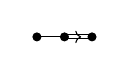
\begin{tikzpicture}
\dynkin{B}{3}
\end{tikzpicture}
\end{tcblisting}
\begin{tcblisting}{title={Indefinite rank Dynkin diagrams}}
\dynkin{B}{}
\end{tcblisting}

\NewDocumentCommand\dyn{mm}%
{%
	\IfStrEq{#2}{}{{#1}_n}{{#1}_{#2}}%
	& \dynkin{#1}{#2} \\
}%

\begin{longtable}{@{}>{$}r<{$}@{ \ }m{\wdt}@{}}
\caption{The Dynkin diagrams of the reduced simple root systems \cite{Bourbaki:2002} pp. 265--290, plates I--IX}\\
\endfirsthead
\caption{(continued)}\\
\endhead
\multicolumn{2}{c}{continued below \dots}
\endfoot
\endlastfoot
\dyn{A}{}
\dyn{B}{}
\dyn{C}{}
\dyn{D}{}
\dyn{E}{6}
\dyn{E}{7}
\dyn{E}{8}
\dyn{F}{4}
\dyn{G}{2}
\end{longtable}

\section{Set options globally}

\begin{tcolorbox}[title={Most options set globally \dots}]
\begin{verbatim}
\pgfkeys{/Dynkin diagram,edgeLength=.5cm,foldradius=.5cm}
\end{verbatim}
\end{tcolorbox}
\begin{tcolorbox}[title={\dots or pass to the package}]
\begin{verbatim}
\usepackage[
     ordering=Kac,
     edge/.style=blue,
     mark=o,
     radius=.06cm]
     {dynkin-diagrams}
\end{verbatim}
\end{tcolorbox}


\section{Coxeter diagrams}

\begin{tcblisting}{title={Coxeter diagram option}}
\dynkin[Coxeter]{F}{4}
\end{tcblisting}

\begin{tcblisting}{title={gonality option for \(G_2\) and \(I_n\) Coxeter diagrams}}
\(G_2=\dynkin[Coxeter,gonality=n]{G}{2}\), \ 
\(I_n=\dynkin[Coxeter,gonality=n]{I}{}\)
\end{tcblisting}

\RenewDocumentCommand\dyn{mm}%
{%
	\IfStrEq{#2}{}%
	{%
		{#1}_n & \dynkin[Coxeter]{#1}{} \\
	}%
	{%
		{#1}_{#2} & \dynkin[Coxeter]{#1}{#2} \\
	}%
}%

\begin{longtable}{@{}>{$}r<{$}@{ \ }m{\wdt}@{}}
\caption{The Coxeter diagrams of the simple reflection groups}\\
\endfirsthead
\caption{(continued)}\\
\endhead
\multicolumn{2}{c}{continued below \dots}
\endfoot
\endlastfoot
\dyn{A}{}
\dyn{B}{}
\dyn{C}{}
\dyn{D}{}
\dyn{E}{6}
\dyn{E}{7}
\dyn{E}{8}
\dyn{F}{4}
G_2 & \dynkin[Coxeter,gonality=n]{G}{2} \\
\dyn{H}{3}
\dyn{H}{4}
I_n & \dynkin[Coxeter,gonality=n]{I}{} \\
\end{longtable}


\section{Satake diagrams}\label{section:Satake}

\begin{tcblisting}{title={Satake diagrams use the standard name instead of a rank}}
\(A_{IIIb}=\dynkin{A}{IIIb}\)
\end{tcblisting}

We use a solid gray bar to denote the folding of a Dynkin diagram, rather than the usual double arrow, since the diagrams turn out simpler and easier to read.

\RenewDocumentCommand\dyn{mm}%
{%
#1_{#2} & \dynkin{#1}{#2} \\
}%

\begin{longtable}{@{}>{$}r<{$}@{ \ }m{\wdt}@{}}
\caption{The Satake diagrams of the real simple Lie algebras \cite{Helgason:2001} p. 532--534}\\
\endfirsthead
\caption{(continued)}\\
\endhead
\multicolumn{2}{c}{continued below \dots}
\endfoot
\endlastfoot
\dyn{A}{I}
\dyn{A}{II}
\dyn{A}{IIIa}
\dyn{A}{IIIb}
\dyn{A}{IV}
\dyn{B}{I}
\dyn{B}{II}
\dyn{C}{I}
\dyn{C}{IIa}
\dyn{C}{IIb}
\dyn{D}{Ia}
\dyn{D}{Ib}
\dyn{D}{Ic}
\dyn{D}{II}
\dyn{D}{IIIa}
\dyn{D}{IIIb}
\dyn{E}{I}
\dyn{E}{II}
\dyn{E}{III}
\dyn{E}{IV}
\dyn{E}{V}
\dyn{E}{VI}
\dyn{E}{VII}
\dyn{E}{VIII}
\dyn{E}{IX}
\dyn{F}{I}
\dyn{F}{II}
\dyn{G}{I}
\end{longtable}


\section{Labels for the roots}

\begin{tcblisting}{title={Label the roots by root number}}
\dynkin[label]{B}{3}
\end{tcblisting}
\begin{tcblisting}{title={Make a macro to assign labels to roots}}
\dynkin[label,labelMacro/.code={\alpha_{#1}}]{D}{5}
\end{tcblisting}
\begin{tcblisting}{title={Make a label for a single root}}
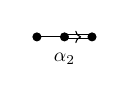
\begin{tikzpicture}
\dynkin{B}{3}
\dynkinLabelRoot{2}{\alpha_2}
\end{tikzpicture}
\end{tcblisting}
\begin{tcblisting}{title={Use a text style}}
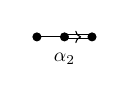
\begin{tikzpicture}
\dynkin[text/.style={scale=1.2}]{B}{3};
\dynkinLabelRoot{2}{\alpha_2}
\end{tikzpicture}
\end{tcblisting}
\begin{tcblisting}{title={Access root labels via TikZ}}
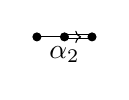
\begin{tikzpicture}
\dynkin{B}{3};
\node[below] at (root 2) {\(\alpha_2\)};
\end{tikzpicture}
\end{tcblisting}
\begin{tcblisting}{title={The labels have default locations}}
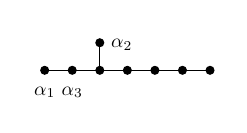
\begin{tikzpicture}
\dynkin{E}{8};
\dynkinLabelRoot{1}{\alpha_1}
\dynkinLabelRoot{2}{\alpha_2}
\dynkinLabelRoot{3}{\alpha_3}
\end{tikzpicture}
\end{tcblisting}
\begin{tcblisting}{title={The starred form flips labels to alternate locations}}
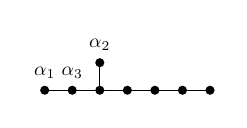
\begin{tikzpicture}
\dynkin{E}{8};
\dynkinLabelRoot*{1}{\alpha_1}
\dynkinLabelRoot*{2}{\alpha_2}
\dynkinLabelRoot*{3}{\alpha_3}
\end{tikzpicture}
\end{tcblisting}

\section{Style}

\begin{tcblisting}{title={Colours}}
\dynkin[edge/.style={blue!50,thick},*/.style=blue!50!red]{F}{4}
\end{tcblisting}
\begin{tcblisting}{title={Edge lengths}}
\dynkin[edgeLength=1.2,parabolic=3]{A}{3}
\end{tcblisting}
\begin{tcblisting}{title={Root marks}}
\dynkin{E}{8}
\dynkin[mark=*]{E}{8}
\dynkin[mark=o]{E}{8}
\dynkin[mark=O]{E}{8}
\dynkin[mark=t]{E}{8}
\dynkin[mark=x]{E}{8}
\dynkin[mark=X]{E}{8}
\end{tcblisting}
At the moment, you can only use:
\par\noindent\begin{tabular}{>{\ttfamily}cl}
* & solid dot \\
o & hollow circle \\
O & double hollow circle \\
t & tensor root \\
x & crossed root \\ 
X & thickly crossed root 
\end{tabular}
\begin{tcblisting}{title={Mark styles}}
\dynkin[parabolic=124,x/.style={brown,very thick}]{E}{8}
\end{tcblisting}
\begin{tcblisting}{title={Sizes of root marks}}
\dynkin[radius=.08cm,parabolic=3]{A}{3}
\end{tcblisting}
\begingroup
\tikzset{/Dynkin diagram,radius=.07cm}
\begin{longtable}{@{}>{$}r<{$}@{ \ }m{\wdt}@{}}
\caption{Classical Lie superalgebras \cite{Frappat/Sciarrino/Sorba:1989}. We need a slightly larger radius parameter to distinguish the tensor product symbols from the solid dots.}\\
\endfirsthead
\caption{(continued)}\\
\endhead
\multicolumn{2}{c}{continued below \dots}
\endfoot
\endlastfoot
A_{mn} & \dynkin{A}{ooo.oto.oo}\\
B_{mn} & \dynkin{B}{ooo.oto.oo}\\
B_{0n} & \dynkin{B}{ooo.ooo.o*}\\
C_{n}  & \dynkin{C}{too.oto.oo}\\
D_{mn} & \dynkin{D}{ooo.oto.oooo}\\
D_{21\alpha} & \dynkin{A}{oto}\\
F_4 & \dynkin{F}{ooot}\\
G_3 & 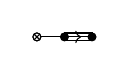
\begin{tikzpicture}[baseline=-0.5ex]\dynkin[extended]{G}{2} \dynkinTensorRootMark{0}\end{tikzpicture}\\
\end{longtable}
\endgroup

\begin{longtable}{@{}>{$}r<{$}@{ \ }m{\wdt}@{}}
\caption{Classical Lie superalgebras \cite{Frappat/Sciarrino/Sorba:1989}. Here we see the problem with using the default radius parameter, which is too small for tensor product symbols.}\\
\endfirsthead
\caption{(continued)}\\
\endhead
\multicolumn{2}{c}{continued below \dots}
\endfoot
\endlastfoot
A_{mn} & \dynkin{A}{ooo.oto.oo}\\
B_{mn} & \dynkin{B}{ooo.oto.oo}\\
B_{0n} & \dynkin{B}{ooo.ooo.o*}\\
C_{n}  & \dynkin{C}{too.oto.oo}\\
D_{mn} & \dynkin{D}{ooo.oto.oooo}\\
D_{21\alpha} & \dynkin{A}{oto}\\
F_4 & \dynkin{F}{ooot}\\
G_3 & 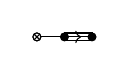
\begin{tikzpicture}[baseline=-0.5ex]\dynkin[extended]{G}{2} \dynkinTensorRootMark{0}\end{tikzpicture}\\
\end{longtable}


\section{Suppress or reverse arrows}

\begin{tcblisting}{title={Some diagrams have double or triple edges}}
\dynkin{F}{4}
\dynkin{G}{2}
\end{tcblisting}
\begin{tcblisting}{title={Suppress arrows}}
\dynkin[arrows=false]{F}{4}
\dynkin[arrows=false]{G}{2}
\end{tcblisting}
\begin{tcblisting}{title={Reverse arrows}}
\dynkin[reverseArrows]{F}{4}
\dynkin[reverseArrows]{G}{2}
\end{tcblisting}


\section{Drawing on top of a Dynkin diagram}

\begin{tcblisting}{title={TikZ can access the roots themselves}}
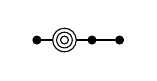
\begin{tikzpicture}
\dynkin{A}{4};
\fill[white,draw=black] (root 2) circle (.15cm);
\fill[white,draw=black] (root 2) circle (.1cm);
\draw[black] (root 2) circle (.05cm);
\end{tikzpicture}
\end{tcblisting}
\begin{tcblisting}{title={Draw curves between the roots}}
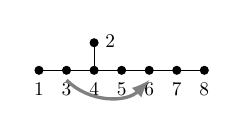
\begin{tikzpicture}
\dynkin[label]{E}{8}
\draw[very thick, black!50,-latex]  
	(root 3.south) to [out=-45, in=-135] (root 6.south); 
\end{tikzpicture}
\end{tcblisting}
\begin{tcblisting}{title={Change marks}}
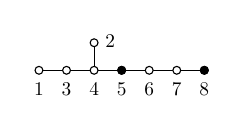
\begin{tikzpicture}
\dynkin[mark=o,label]{E}{8};
\dynkinRootMark{*}{5}
\dynkinRootMark{*}{8}
\end{tikzpicture}
\end{tcblisting}


\section{Mark lists}

The package allows a list of root marks instead of a rank:

\begin{tcblisting}{title={A mark list}}
\dynkin{E}{oo**ttxx}
\end{tcblisting}
The mark list \verb!oo**ttxx! has one mark for each root: \verb!o!, \verb!o!, \dots, \verb!x!.
Roots are listed in the current default ordering.
(Careful: in an affine root system, a mark list will \emph{not} contain a mark for root zero.)


\section{Indefinite edges}

An \emph{indefinite edge} is a dashed edge between two roots, \dynkin{A}{*.*} indicating that an indefinite number of roots have been omitted from the Dynkin diagram.
In between any two entries in a mark list, place a period to indicate an indefinite edge:
\begin{tcblisting}{title={Indefinite edges}}
\dynkin{D}{o.o*.*.t.to.t}
\end{tcblisting}

In certain diagrams, roots may have an edge between them even though they are not subsequent in the ordering.
For such rare situations, there is an option:
\begin{tcblisting}{title={Indefinite edge option}}
\dynkin[makeIndefiniteEdge={3-5},label]{D}{5}
\end{tcblisting}
\begin{tcblisting}{title={Give a list of edges to become indefinite}}
\dynkin[makeIndefiniteEdge/.list={1-2,3-5},label]{D}{5}
\end{tcblisting}

\begin{tcblisting}{title={Indefinite edge style}}
\dynkin[indefiniteEdge/.style={draw=black,fill=white,thin,densely dashed},%
	edgeLength=1cm,%
	makeIndefiniteEdge={3-5}]
	{D}{5}
\end{tcblisting}

\begin{tcblisting}{title={The ratio of the lengths of indefinite edges to those of other edges}}
\dynkin[edgeLength = .5cm,%
	indefiniteEdgeRatio=3,%
	makeIndefiniteEdge={3-5}]
	{D}{5}
\end{tcblisting}


\section{Parabolic subgroups}

Each set of roots is assigned a number, with each binary digit zero or one to say whether the corresponding root is crossed or not:
\begin{tcblisting}{}
The flag variety of pointed lines in 
projective 3-space is associated to 
the Dynkin diagram \dynkin[parabolic=3]{A}{3}.
\end{tcblisting}

\renewcommand*{\arraystretch}{1.5}
\begin{longtable}{@{}>{$}r<{$}m{2.5cm}m{5cm}@{}}
\caption{The Hermitian symmetric spaces}
\endfirsthead
\caption{(continued)}
\endhead
\multicolumn{2}{c}{continued below \dots}
\endfoot
\endlastfoot
  A_n &
  \dynkin{A}{**.*x*.**} & 
  Grassmannian of $k$-planes in $\C{n+1}$ 
  \\
  B_n &
  \dynkin[parabolic=1]{B}{} & 
  $(2n-1)$-dimensional hyperquadric, i.e. the variety of null lines in $\C{2n+1}$
  \\
  C_n &
  \dynkin[parabolic=16]{C}{} & 
  space of Lagrangian $n$-planes in $\C{2n}$
  \\
 D_n &
 \dynkin[parabolic=1]{D}{} & 
 $(2n-2)$-dimensional hyperquadric, i.e. the variety of null lines in $\C{2n}$
 \\
 D_n &
 \dynkin[parabolic=32]{D}{} & 
  one component of the variety of maximal dimension null subspaces of $\C{2n}$ \\
  D_n &
  \dynkin[parabolic=16]{D}{} & 
  the other component\\
  E_6 &
  \dynkin[parabolic=1]{E}{6} &
  complexified octave projective plane\\
  E_6 & 
  \dynkin[parabolic=32]{E}{6}&its dual plane\\ 
 E_7 &
 \dynkin[parabolic=64]{E}{7}& the space of null octave 3-planes in octave 6-space
\end{longtable}


\section{Extended Dynkin diagrams}

\begin{tcblisting}{title={Extended Dynkin diagrams}}
\dynkin[extended]{A}{7}
\end{tcblisting}


The extended Dynkin diagrams are also described in the notation of Kac \cite{Kac:1990} p. 55 as affine untwisted Dynkin diagrams: we extend \verb!\dynkin{A}{7}! to become \verb!\dynkin{A}[1]{7}!:
\begin{tcblisting}{title={Extended Dynkin diagrams}}
\dynkin{A}[1]{7}
\end{tcblisting}

\RenewDocumentCommand\dyn{mm}%
{%
	\IfStrEq{#2}{}{\tilde{#1}_n}{	\tilde{#1}_{#2}}%
	 & \dynkin[extended]{#1}{#2} \\
}%

\begin{longtable}{@{}>{$}r<{$}@{ \ }m{\wdt}@{}}
\caption{The Dynkin diagrams of the extended simple root systems}\\
\endfirsthead
\caption{(continued)}\\
\endhead
\multicolumn{2}{c}{continued below \dots}
\endfoot
\endlastfoot
\dyn{A}{1}
\dyn{A}{}
\dyn{B}{}
\dyn{C}{}
\dyn{D}{}
\dyn{E}{6}
\dyn{E}{7}
\dyn{E}{8}
\dyn{F}{4}
\dyn{G}{2}
\end{longtable}


\section{Affine twisted and untwisted Dynkin diagrams}

The affine Dynkin diagrams are described in the notation of Kac \cite{Kac:1990} p. 55:
\begin{tcblisting}{title={Affine Dynkin diagrams}}
\(A^{(1)}_7=\dynkin{A}[1]{7}, \ 
E^{(2)}_6=\dynkin{E}[2]{6}, \ 
D^{(3)}_4=\dynkin{D}[3]{4}\)
\end{tcblisting}


\RenewDocumentCommand\dyn{mmm}%
{%
	\IfStrEqCase{#3}%
	{%
		{}%
		{%
			{#1}^{#2}_{\ell} & \dynkin[label,name={#1-#2}]{#1}[#2]{} \\
		}%
		{odd}%
		{%
			{#1}^2_{2\ell-1} & \dynkin[label,name={#1-#2-odd}]{#1}[#2]{#3} \\
		}%
		{even}%
		{%
			{#1}^2_{2\ell} & \dynkin[label,name={#1-#2-even}]{#1}[#2]{#3} \\
		}%
	}%
	[{{#1}^{#2}_{#3} & \dynkin[label,name={#1-#2-#3}]{#1}[#2]{#3} \\}]
}%

\begin{longtable}{@{}>{$}r<{$}@{ \ }m{\wdt}@{}}
\caption{The affine Dynkin diagrams}\\
\endfirsthead
\caption{(continued)}\\
\endhead
\multicolumn{2}{c}{continued below \dots}
\endfoot
\endlastfoot
\dyn{A}{1}{1}
\dyn{A}{1}{}
\dyn{B}{1}{}
\dyn{C}{1}{}
\dyn{D}{1}{}
\dyn{E}{1}{6}
\dyn{E}{1}{7}
\dyn{E}{1}{8}
\dyn{F}{1}{4}
\dyn{G}{1}{2}
\dyn{A}{2}{2}
\dyn{A}{2}{even}
\dyn{A}{2}{odd}
\dyn{D}{2}{}
\dyn{E}{2}{6}
\dyn{D}{3}{4}
\end{longtable}

\begin{longtable}{@{}>{$}r<{$}@{ \ }m{\wdt}@{}}
\caption{Some more affine Dynkin diagrams}\\
\endfirsthead
\caption{(continued)}\\
\endhead
\multicolumn{2}{c}{continued below \dots}
\endfoot
\endlastfoot
\dyn{A}{2}{4}
\dyn{A}{2}{5}
\dyn{A}{2}{6}
\dyn{A}{2}{7}
\dyn{A}{2}{8}
\dyn{D}{2}{3}
\dyn{D}{2}{4}
\dyn{D}{2}{5}
\dyn{D}{2}{6}
\dyn{D}{2}{7}
\dyn{D}{2}{8}
\dyn{D}{3}{4}
\dyn{E}{2}{6}
\end{longtable}


\section{Extended Coxeter diagrams}

\begin{tcblisting}{title={Extended and Coxeter options together}}
\dynkin[extended,Coxeter]{F}{4}
\end{tcblisting}

\RenewDocumentCommand\dyn{mm}%
{%
	\IfStrEq{#2}{}{\tilde{#1}_n}{\tilde{#1}_{#2}}%
	 & \dynkin[extended,Coxeter]{#1}{#2} \\
}%

\begin{longtable}{@{}>{$}r<{$}@{ \ }m{\wdt}@{}}
\caption{The extended (affine) Coxeter diagrams}\\
\endfirsthead
\caption{(continued)}\\
\endhead
\multicolumn{2}{c}{continued below \dots}
\endfoot
\endlastfoot
\dyn{A}{}
\dyn{B}{}
\dyn{C}{}
\dyn{D}{}
\dyn{E}{6}
\dyn{E}{7}
\dyn{E}{8}
\dyn{F}{4}
G_2 & \dynkin[extended,Coxeter]{G}{2} \\
\dyn{H}{3}
\dyn{H}{4}
\dyn{I}{1}
\end{longtable}


\section{Kac style}

We include a style called \verb!Kac! which tries to imitate the style of \cite{Kac:1990}.

\begin{tcblisting}{title={Kac style}}
\dynkin[Kac]{F}{4}
\end{tcblisting}


\RenewDocumentCommand\dyn{mm}%
{%
	\IfStrEq{#2}{}{\tilde{#1}_n}{	\tilde{#1}_{#2}}%
	 & \dynkin[extended]{#1}{#2} \\
}%

\begingroup
\pgfkeys{/Dynkin diagram,Kac}
\begin{longtable}{@{}>{$}r<{$}@{ \ }m{\wdt}@{}}
\caption{The Dynkin diagrams of the extended simple root systems in Kac style}\\
\endfirsthead
\caption{(continued)}\\
\endhead
\multicolumn{2}{c}{continued below \dots}
\endfoot
\endlastfoot
\dyn{A}{1}
\dyn{A}{}
\dyn{B}{}
\dyn{C}{}
\dyn{D}{}
\dyn{E}{6}
\dyn{E}{7}
\dyn{E}{8}
\dyn{F}{4}
\dyn{G}{2}
\end{longtable}
\endgroup



\section{Folded Dynkin diagrams}

The Dynkin diagrams package has limited support for folding Dynkin diagrams.

\begin{tcblisting}{title={Folding}}
\dynkin[fold]{A}{13}
\end{tcblisting}

\begin{tcblisting}{title={Big fold radius}}
\dynkin[fold,foldradius=1cm]{A}{13}
\end{tcblisting}

\begin{tcblisting}{title={Small fold radius}}
\dynkin[fold,foldradius=.2cm]{A}{13}
\end{tcblisting}

Some Dynkin diagrams have multiple foldings, which we attempt to distinguish (not entirely successfully) by their \emph{ply}: the maximum number of roots folded together.
Most diagrams can only allow a 2-ply folding, so \verb!fold! is a synonym form \verb!ply=2!.

\begin{tcblisting}{title={3-ply}}
\dynkin[ply=3]{D}{4}
\dynkin[ply=3]{D}[1]{4}
\end{tcblisting}

\begin{tcblisting}{title={4-ply}}
\dynkin[ply=4]{D}[1]{4}
\end{tcblisting}

The \(D^{(1)}_{\ell}\) diagrams can be folded on their left end and separately on their right end:
\begin{tcblisting}{title={Left, right and both}}
\dynkin{D}[1]{} \
\dynkin[foldleft]{D}[1]{} \
\dynkin[foldright]{D}[1]{} \
\dynkin[fold]{D}[1]{}
\end{tcblisting}

We have to be careful about the 4-ply foldings of \(D^{(1)}_{2\ell}\), for which we can have two different patterns, so by default, the package only draws as much as it can without distinguishing the two:
\begin{tcblisting}{title={Default \(D^{(1)}_{2\ell}\) and the two ways to finish it}}
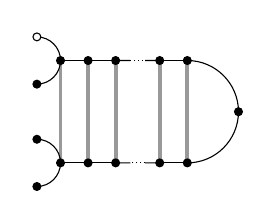
\begin{tikzpicture}
\dynkin[ply=4]{D}[1]{****.*****.*****}%
\end{tikzpicture} \ 
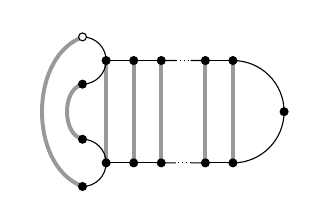
\begin{tikzpicture}
\dynkin[ply=4]{D}[1]{****.*****.*****}%
\dynkinFold[bend right=65]{1}{13}%
\dynkinFold[bend right=65]{0}{14}%
\end{tikzpicture} \ 
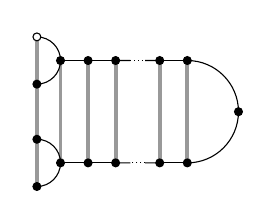
\begin{tikzpicture}
\dynkin[ply=4]{D}[1]{****.*****.*****}%
\dynkinFold{0}{1}%
\dynkinFold{1}{13}%
\dynkinFold{13}{14}%
\end{tikzpicture}
\end{tcblisting}



\begingroup
\NewDocumentCommand\seriesName{mmm}%
{%
	\IfStrEq{#2}{0}{#1_{#3}}{#1^{#2}_{#3}}%
}%
\NewDocumentCommand\foldingTable{smmmmmmmm}%
{%
\begin{tcolorbox}[width=5cm]
\begin{tabular}{@{}>{$}r<{$}@{}m{\wdt}@{}}%
\seriesName{#2}{#3}{#4}&#5\\
\seriesName{#6}{#7}{#8}&\IfBooleanTF{#1}{\reflectbox{#9}}{#9}%
\end{tabular}%
\end{tcolorbox}
}%


\NewDocumentCommand\fold{smmmmmm}%
{%
	\IfBooleanTF{#1}%
	{%
		\foldingTable*%
		{#2}{#3}{#4}{\dynkin[fold]{#2}[#3]{#4}}%
		{#5}{#6}{#7}{\dynkin{#5}[#6]{#7}}%
	}%
	{%
		\foldingTable%
		{#2}{#3}{#4}{\dynkin[fold]{#2}[#3]{#4}}%
		{#5}{#6}{#7}{\dynkin{#5}[#6]{#7}}%
	}%
}%

\pgfkeys{/Dynkin diagram,foldradius=.35cm}
\begin{longtable}{@{}l@{}}
\caption{Some foldings of Dynkin diagrams}\\
\endfirsthead
\caption{(continued)}\\
\endhead
\multicolumn{1}{c}{continued below \dots}
\endfoot
\endlastfoot
\fold{A}{0}{3}{C}{0}{2}
\\
\foldingTable{A}{0}{2\ell-1}{\dynkin[fold]{A}{**.*****.**}}%
{C}{0}{\ell}{\dynkin{C}{}}
\\
\fold*{B}{0}{3}{G}{0}{2}
\\
\foldingTable{D}{0}{4}{\dynkin[ply=3]{D}{4}}%
{G}{0}{2}{\dynkin{G}{2}}
\\
\foldingTable{D}{0}{\ell+1}{\dynkin[fold]{D}{}}%
{B}{0}{\ell}{\dynkin{B}{}}
\\
\fold*{E}{0}{6}{F}{0}{4}
\\
\foldingTable{A}{1}{3}{\dynkin[ply=4]{A}[1]{3}}%
{A}{1}{1}{\dynkin{A}[1]{1}}
\\
\foldingTable{A}{1}{2\ell-1}{\dynkin[fold]{A}[1]{**.*****.**}}%
{C}{1}{\ell}{\dynkin{C}[1]{}}
\\
\foldingTable{B}{1}{3}{\dynkin[ply=3]{B}[1]{3}}%
{A}{2}{2}{\dynkin{A}[2]{2}}
\\
\foldingTable{B}{1}{3}{\dynkin[ply=2]{B}[1]{3}}%
{G}{1}{2}{\dynkin{G}[1]{2}}
\\
\foldingTable{B}{1}{\ell}{\dynkin[fold]{B}[1]{}}{D}{2}{\ell}{\dynkin{D}[2]{}}
\\
\foldingTable{D}{1}{4}{\dynkin[ply=3]{D}[1]{4}}%
{B}{1}{3}{\dynkin{B}[1]{3}}
\\
\foldingTable{D}{1}{4}{\dynkin[ply=3]{D}[1]{4}}%
{G}{1}{2}{\dynkin{G}[1]{2}}
\\
\foldingTable{D}{1}{\ell+1}{\dynkin[fold]{D}[1]{}}%
{D}{2}{\ell}{\dynkin{D}[2]{}}
\\
\foldingTable{D}{1}{\ell+1}{%
\dynkin[foldright]{D}[1]{}}%
{B}{1}{\ell}{\dynkin{B}[1]{}}
\\
\foldingTable{D}{1}{2\ell}{%
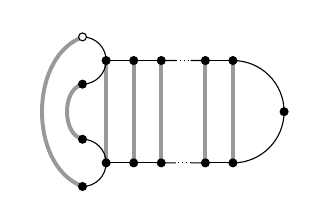
\begin{tikzpicture}
\dynkin[ply=4]{D}[1]{****.*****.*****}%
\dynkinFold[bend right=65]{1}{13}%
\dynkinFold[bend right=65]{0}{14}%
\end{tikzpicture}
}%
{A}{2}{\text{odd}}{\dynkin{A}[2]{odd}}
\\
\foldingTable{D}{1}{2\ell}{%
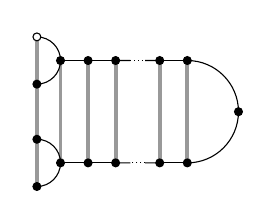
\begin{tikzpicture}
\dynkin[ply=4]{D}[1]{****.*****.*****}%
\dynkinFold{0}{1}%
\dynkinFold{1}{13}%
\dynkinFold{13}{14}%
\end{tikzpicture}
}%
{A}{2}{\text{even}}{\dynkin{A}[2]{even}}
\\
\fold*{E}{1}{6}{F}{1}{4}
\\
\foldingTable{E}{1}{6}{\dynkin[ply=3]{E}[1]{6}}%
{D}{3}{4}{\dynkin{D}[3]{4}}
\\
\fold{E}{1}{7}{E}{2}{6}
\\
\fold{F}{1}{4}{G}{1}{2}
\\
\foldingTable{A}{2}{\text{odd}}{%
\dynkin[odd,fold]{A}[2]{****.***}
}%
{A}{2}{\text{even}}{\dynkin{A}[2]{even}}
\\
\foldingTable{D}{2}{3}{\dynkin[fold]{D}[2]{3}}%
{A}{2}{2}{\dynkin{A}[2]{2}}
\\
\end{longtable}
\endgroup



\section{Root ordering}\label{section:order}

\begin{tcblisting}{title={Root ordering}}
\dynkin[ordering=Adams]{E}{6}
\dynkin[ordering=Bourbaki]{E}{6}
\dynkin[ordering=Carter]{E}{6}
\dynkin[ordering=Dynkin]{E}{6}
\dynkin[ordering=Kac]{E}{6}
\end{tcblisting}
Default is Bourbaki.

\NewDocumentCommand\tablerow{mm}%
{%
\(#1_{#2}\)
&
\dynkin[label,ordering=Adams]{#1}{#2}
&
\dynkin[label]{#1}{#2}
&
\dynkin[label,ordering=Carter]{#1}{#2}
&
\dynkin[label,ordering=Dynkin]{#1}{#2}
&
\dynkin[label,ordering=Kac]{#1}{#2}
\\
}%

\begin{center}
\begin{longtable}{@{}llllll@{}}
\toprule
& Adams & Bourbaki & Carter & Dynkin & Kac \\ \midrule
\endfirsthead
\toprule
Adams & Bourbaki & Carter & Dynkin & Kac \\ \midrule
\endhead
\bottomrule
\endfoot
\bottomrule
\endlastfoot
\tablerow{E}{6}
\tablerow{E}{7}
\tablerow{E}{8}
\tablerow{F}{4}
\tablerow{G}{2}
\end{longtable}
\end{center}


\section{Naming Dynkin diagrams and connecting different ones}\label{section:name}

We can make some sophisticated folded diagrams by drawing multiple diagrams, each with a name:
\begin{tcblisting}{title={Name a diagram}}
\dynkin[name=Bob]{D}{6}
\end{tcblisting}
We can then connect the two with folding edges:
\begin{tcblisting}{title={Connect diagrams}}
\begin{tikzpicture}
\dynkin[name=upper]{A}{3}
\dynkin[name=lower]{A}{3}
\foreach \i in {1,...,3}%
{%
	\draw[/Dynkin diagram/foldStyle] ($(upper root \i)$) -- ($(lower root \i)$);%
}%
\end{tikzpicture}
\end{tcblisting}

The following diagrams arise in the Satake diagrams of the pseudo-Riemannian symmetric spaces \cite{Baba:2009}.

\par\noindent\begingroup
\pgfkeys{/Dynkin diagram,edgeLength=.5cm,foldradius=.5cm}
\begin{tikzpicture}
\foreach \d in {1,...,2}
{
	\node (current) at ($(0,\d*.4)$){};
	\dynkin[name=\d,at=(current)]{A}{IIIb}
}
\begin{scope}[on background layer]
\foreach \i in {1,...,6}%
{%
	\draw[/Dynkin diagram/foldStyle] ($(1 root \i)$) -- ($(2 root \i)$);%
}%
\end{scope}
\end{tikzpicture}
\endgroup

\par\noindent\begingroup
\pgfkeys{/Dynkin diagram/edgeLength=.75cm,/Dynkin diagram/edge/.style={draw=white,double=black,very thick},
}
\begin{tikzpicture}
\foreach \d in {1,...,4}
{
	\node (current) at ($(0,\d*.3)$){};
	\dynkin[name=\d,at=(current)]{D}{oo.oooo}
}
\begin{scope}[on background layer]
\foreach \i in {1,...,6}%
{%
	\draw[/Dynkin diagram/foldStyle] ($(1 root \i)$) -- ($(2 root \i)$);%
	\draw[/Dynkin diagram/foldStyle] ($(2 root \i)$) -- ($(3 root \i)$);%
	\draw[/Dynkin diagram/foldStyle] ($(3 root \i)$) -- ($(4 root \i)$);%
}%
\end{scope}
\end{tikzpicture}
\endgroup


\section{Other examples}


\begingroup

\NewDocumentCommand\labls{m}%
{%
	\ifcase#1%
		{1}\or%
		{1}\or%
		{2}\or%
		{2}\or%
		{2}\or%
		{2}\or%
		{2}\or%
		{1}\or%
		{1}\or%
		\else\typeout{What?}%
		\fi%
}%
\NewDocumentCommand\lablIt{m}%
{%
	\ifnum#1=0\relax%
		1%
	\else
		2%
	\fi%
}%


\tikzset{/Dynkin diagram,labelMacro/.code=\labls{#1},label,radius=.06cm}

\NewDocumentCommand\FfourOneReal{m}%
{%
	\begin{tikzpicture}%
		\dynkin{A}{#1}%
		\dynkinQuadrupleEdge{1}{2}%
		\dynkinTripleEdge{4}{3}%
	\end{tikzpicture}%
}%

\NewDocumentCommand\GtwoOneReal{m}%
{%
	\begin{tikzpicture}%
		\dynkin{A}{#1}%
		\dynkinQuadrupleEdge{1}{2}%
		\dynkinDefiniteDoubleEdge{4}{3}%
	\end{tikzpicture}%
}%

\begin{longtable}{@{}>{$}r<{$}m{5cm}@{}}
\caption{The Vogan diagrams of some affine Lie superalgebras \cite{Ransingh:2013,Ransingh:unpub}}%
\endfirsthead
\caption{(continued)}
\endhead
\text{continued below \dots}
\endfoot
\endlastfoot
\mathfrak{sl}\left(2m|2n\right)^{(2)} &
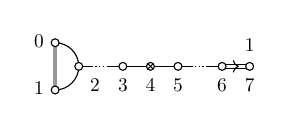
\begin{tikzpicture}
\dynkin[ply=2,label]{B}[1]{oo.oto.oo}
\dynkinLabelRoot*{7}{1}
\end{tikzpicture}
\\
&\dynkin[label]{B}[1]{oo.oto.oo}\\
&\dynkin[ply=2,label]{B}[1]{oo.Oto.Oo}\\
&\dynkin[label]{B}[1]{oo.Oto.Oo}\\
&\dynkin[label]{D}[1]{oo.oto.ooo}\\
&\dynkin[label]{D}[1]{oO.otO.ooo}\\
&\dynkin[label,fold]{D}[1]{oo.oto.ooo}\\
\mathfrak{sl}\left(2m+1|2n\right)^2 &
\dynkin[label]{B}[1]{oo.oto.oo}\\
&\dynkin[label]{B}[1]{oO.oto.oO}\\
&\dynkin[label,fold]{B}[1]{oo.oto.oo}\\
\mathfrak{sl}\left(2m+1|2n+1\right)^2
&\dynkin[label]{D}[2]{o.oto.oo}\\
&\dynkin[label]{D}[2]{o.OtO.oo}\\
\mathfrak{sl}\left(2|2n+1\right)^{(2)}
&\dynkin[ply=2,label,doubleEdges]{B}[1]{oo.Oto.Oo}\\
&\dynkin[ply=2,label,doubleFold]{B}[1]{oo.Oto.Oo}\\
&\dynkin[ply=2,label,doubleEdges]{B}[1]{oo.OtO.oo}\\
&\dynkin[ply=2,label,doubleFold]{B}[1]{oo.OtO.oo}\\
\mathfrak{sl}\left(2|2n\right)^{(2)}
&\dynkin[ply=2,label,doubleEdges]{D}[1]{oo.oto.ooo}\\
&\dynkin[ply=2,label,doubleFoldLeft]{D}[1]{oo.oto.ooo}\\
\mathfrak{osp}\left(2m|2n\right)^{(2)}
&\dynkin[label,labelMacro/.code={1}]{D}[2]{o.oto.oo}\\
&\dynkin[label,labelMacro/.code={1}]{D}[2]{o.Oto.Oo}\\
\mathfrak{osp}\left(2|2n\right)^{(2)}
&\dynkin[label,labelMacro/.code=\lablIt{#1},affineMark=*]{D}[2]{o.o.o.o*}\\
&\dynkin[label,labelMacro/.code=\lablIt{#1},affineMark=*]{D}[2]{o.O.o.o*}\\
\mathfrak{sl}\left(1|2n+1\right)^{4}
&\dynkin[label,labelMacro/.code={1}]{D}[2]{o.o.o.o*}\\
&\dynkin[label,labelMacro/.code={1}]{D}[2]{o.o.O.o*}\\
A^1&
\begin{tikzpicture}
\dynkin[name=upper]{A}{oo.t.oo}
\node (Dynkin current) at (upper root 1){};
\dynkinSouth
\dynkin[at=(Dynkin current),name=lower]{A}{oo.t.oo}
\begin{scope}[on background layer]
\foreach \i in {1,...,5}{
	\draw[/Dynkin diagram/foldStyle] ($(upper root \i)$) -- ($(lower root \i)$);
}
\end{scope}
\end{tikzpicture}
\\
&\dynkin[fold]{A}[1]{oo.t.ooooo.t.oo}
\\
&\dynkin[fold,affineMark=t]{A}[1]{oo.o.ootoo.o.oo}
\\
&\dynkin[affineMark=t]{A}[1]{o*.t.*o}
\\
B^1&
\dynkin[affineMark=*]{A}[2]{o.oto.o*}
\\
&\dynkin[affineMark=*]{A}[2]{o.oto.o*}
\\
&\dynkin[affineMark=*]{A}[2]{o.ooo.oo}
\\
&\dynkin[odd]{A}[2]{oo.*to.*o}
\\
&\dynkin[odd,fold]{A}[2]{oo.oto.oo}
\\
&\dynkin[odd,fold]{A}[2]{o*.oto.o*}
\\
D^1&
\dynkin{D}{otoo}
\\
&\dynkin{D}{ot*o}
\\
&\dynkin[fold]{D}{otoo}
\\
C^1&
\dynkin[doubleEdges,fold,affineMark=t,odd]{A}[2]{to.o*}
\\
&\dynkin[doubleEdges,fold,affineMark=t,odd]{A}[2]{t*.oo}
\\
F^1&
\FfourOneReal{oto*}
\\
&
\FfourOneReal{*too}
\\
G^1
&\GtwoOneReal{ot*oo}\\
&\GtwoOneReal{oto*o}\\
&\GtwoOneReal{*too*}\\
&\GtwoOneReal{*tooo}\\
\end{longtable}
\endgroup



\section{Syntax}

The syntax is \verb!\dynkin[<options>]{<letter>}[<twisted rank>]{<rank>}! where \verb!<letter>! is \(A,B,C,D,E,F\) or \(G\), the family of root system for the Dynkin diagram, \verb!<twisted rank>! is \(0,1,2,3\) (default is 0) representing:
\[
\begin{array}{rp{3cm}}
0 & finite root system \\
1 & affine extended root system, i.e.  of type \({}^{(1)}\) \\
2 & affine twisted root system of type \({}^{(2)}\) \\
3 & affine twisted root system of type \({}^{(3)}\) \\
\end{array}
\]
and \verb!<rank>! is 
\begin{enumerate}
\item
an integer representing the rank or 
\item
blank to represent an indefinite rank or
\item
the name of a Satake diagram as in section~\ref{section:Satake}.
\end{enumerate}



\section{Options}

\newcommand*{\typ}[1]{\(\left<\texttt{#1}\right>\)}
\newcommand*{\optionLabel}[3]{%%
\multicolumn{2}{l}{\(\texttt{#1}=\texttt{#2}\),} \\
\multicolumn{2}{l}{\(\textrm{default}: \texttt{#3}\)} \\
}%%


\par\noindent%
\begin{longtable}{p{1cm}p{10cm}}
\endfirsthead
%\caption{(continued)}\\
\endhead
%\multicolumn{2}{c}{continued below \dots}
\endfoot
\endlastfoot
\optionLabel{text/.style}{\typ{TikZ style data}}{scale=.7}
& Style for any labels on the roots. \\
\optionLabel{name}{\typ{string}}{anonymous}
& A name for the Dynkin diagram, with \texttt{anonymous} treated as a blank; see section~\ref{section:name}. \\
\optionLabel{parabolic}{\typ{integer}}{0} 
& A parabolic subgroup with specified integer, where the integer
is computed as \(n=\sum 2^{i-1} a_i\), \(a_i=0\) or \(1\), to say that root \(i\) is crossed, i.e. a noncompact root. \\
\optionLabel{radius}{\typ{number}cm}{.05cm}
&      size of the dots and of the crosses in the Dynkin diagram \\
\optionLabel{edgeLength}{\typ{number}cm}{.35cm}
&      distance between nodes in the Dynkin diagram \\
\optionLabel{edge/.style}{TikZ style data}{thin}
&      style of edges in the Dynkin diagram \\
\optionLabel{mark}{\typ{o,O,t,x,X,*}}{*}
&      default root mark \\
\optionLabel{affineMark}{o,O,t,x,X,*}{*}
&      default root mark for root zero in an affine Dynkin diagram \\
\optionLabel{label}{true or false}{false}
& whether to label the roots according to the current labelling scheme. \\
\optionLabel{labelMacro}{\typ{1-parameter \TeX{} macro}}{\texttt{\#1}}
& the current labelling scheme. \\
\optionLabel{makeIndefiniteEdge}{\typ{edge pair \(i\)-\(j\) or list of such}}{\{\}}
& edge pair or list of edge pairs to treat as having indefinitely many roots on them. \\
\optionLabel{indefiniteEdgeRatio}{\typ{float}}{1.6}
& ratio of indefinite edge lengths to other edge lengths. \\
\optionLabel{indefiniteEdge/.style}{\typ{TikZ style data}}{draw=black,fill=white,thin,densely dotted}
& style of the dotted or dashed middle third of each indefinite edge. \\
\optionLabel{arrows}{\typ{true or false}}{true}
& whether to draw the arrows that arise along the edges. \\
\optionLabel{reverseArrows}{\typ{true or false}}{true}
& whether to reverse the direction of the arrows that arise along the edges. \\
\optionLabel{fold}{\typ{true or false}}{true}
& whether, when drawing Dynkin diagrams, to draw them 2-ply. \\
\optionLabel{ply}{\typ{0,1,2,3,4}}{0}
& how many roots get folded together, at most. \\
\optionLabel{foldleft}{\typ{true or false}}{true}
& whether to fold the roots on the left side of a Dynkin diagram. \\
\optionLabel{foldright}{\typ{true or false}}{true}
& whether to fold the roots on the right side of a Dynkin diagram. \\
\optionLabel{foldradius}{\typ{length}}{.3cm}
& the radius of circular arcs used in curved edges of folded Dynkin diagrams. \\
\optionLabel{foldStyle}{\typ{TikZ style data}}{draw=black!40,fill=none,line width=radius}
& when drawing folded diagrams, style for the fold indicators. \\
\optionLabel{*/.style}{\typ{TikZ style data}}{draw=black,fill=black}
& style for roots like \dynkin{A}{*} \\
\optionLabel{o/.style}{\typ{TikZ style data}}{draw=black,fill=black}
& style for roots like \dynkin{A}{o}  \\
\optionLabel{O/.style}{\typ{TikZ style data}}{draw=black,fill=black}
& style for roots like \dynkin{A}{O}  \\
\optionLabel{t/.style}{\typ{TikZ style data}}{draw=black,fill=black}
& style for roots like \dynkin{A}{t} \\
\optionLabel{x/.style}{\typ{TikZ style data}}{draw=black}
& style for roots like \dynkin{A}{x}  \\
\optionLabel{X/.style}{\typ{TikZ style data}}{draw=black,thick}
& style for roots like \dynkin{A}{X} \\
\optionLabel{leftFold/.style}{\typ{TikZ style data}}{}
& style to override the \texttt{fold} style when folding roots together on the left half of a Dynkin diagram \\
\optionLabel{rightFold/.style}{\typ{TikZ style data}}{}
& style to override the \texttt{fold} style when folding roots together on the right half of a Dynkin diagram \\
\optionLabel{doubleEdges}{\typ{}}{not set}
& set to override the \texttt{fold} style when folding roots together in a Dynkin diagram, so that the foldings
are indicated with double edges (like those of an \(F_4\) Dynkin diagram without arrows). \\
\optionLabel{doubleFold}{\typ{}}{not set}
& set to override the \texttt{fold} style when folding roots together in a Dynkin diagram, so that the foldings
are indicated with double edges (like those of an \(F_4\) Dynkin diagram without arrows), but filled in solidly. \\
\optionLabel{doubleLeft}{\typ{}}{not set}
& set to override the \texttt{fold} style when folding roots together at the left side of a Dynkin diagram, so that the foldings are indicated with double edges (like those of an \(F_4\) Dynkin diagram without arrows). \\
\optionLabel{doubleFoldLeft}{\typ{}}{not set}
& set to override the \texttt{fold} style when folding roots together  at the left side of a Dynkin diagram, so that the foldings are indicated with double edges (like those of an \(F_4\) Dynkin diagram without arrows), but filled in solidly. \\
\optionLabel{doubleRight}{\typ{}}{not set}
& set to override the \texttt{fold} style when folding roots together at the right side of a Dynkin diagram, so that the foldings are indicated with double edges (like those of an \(F_4\) Dynkin diagram without arrows). \\
\optionLabel{doubleFoldRight}{\typ{}}{not set}
& set to override the \texttt{fold} style when folding roots together  at the right side of a Dynkin diagram, so that the foldings are indicated with double edges (like those of an \(F_4\) Dynkin diagram without arrows), but filled in solidly.
\\
\optionLabel{Coxeter}{\typ{true or false}}{false}
& whether to draw a Coxeter diagram, rather than a Dynkin diagram. \\
\optionLabel{ordering}{\typ{Adams, Bourbaki, Carter, Dynkin, Kac}}{Bourbaki}
& which ordering of the roots to use in exceptional root systems as in section~\ref{section:order}. \\
\end{longtable}
\par\noindent{}All other options are passed to TikZ.


\nocite{*}
\bibliographystyle{amsplain}
\bibliography{dynkin-diagrams}
\end{document}
